\documentclass{beamer}

\newcommand{\chapterframe}[1]{\begin{frame}\centering\huge{#1}\end{frame}}
\newcommand{\mt}[1]{\textnormal{#1}}

\title{Quantum Computing}
\subtitle{Introduction \& recent developments}
\author{Stephan Spindler \and Janos Tapolczai \and Dominik Theuerkauf}


\mode<presentation>
{
  \usetheme{Pittsburgh}      % or try Darmstadt, Madrid, Warsaw, ...
  \usecolortheme{crane} % or try albatross, beaver, crane, ...
  \usefonttheme{default}  % or try serif, structurebold, ...
  \setbeamertemplate{navigation symbols}{}
  \setbeamertemplate{headline}{}
  \setbeamertemplate{caption}[numbered]
  \setbeamertemplate{footline}[frame number]
} 

\setbeamerfont{page number in head/foot}{size=\large}


\usepackage{listings}
\usepackage[english]{babel}
\usepackage[utf8x]{inputenc}
\usepackage{braket}
\usepackage{amsmath,amssymb}
\usepackage{graphicx}
\usepackage{dsfont,bbm}

\newtheorem{code}[theorem]{Code}

%input by dt 4 drawing quantum circuits
%    Q-circuit version 2
%    Copyright (C) 2004  Steve Flammia & Bryan Eastin
%    Last modified on: 9/16/2011
%
%    This program is free software; you can redistribute it and/or modify
%    it under the terms of the GNU General Public License as published by
%    the Free Software Foundation; either version 2 of the License, or
%    (at your option) any later version.
%
%    This program is distributed in the hope that it will be useful,
%    but WITHOUT ANY WARRANTY; without even the implied warranty of
%    MERCHANTABILITY or FITNESS FOR A PARTICULAR PURPOSE.  See the
%    GNU General Public License for more details.
%
%    You should have received a copy of the GNU General Public License
%    along with this program; if not, write to the Free Software
%    Foundation, Inc., 59 Temple Place, Suite 330, Boston, MA  02111-1307  USA

% Thanks to the Xy-pic guys, Kristoffer H Rose, Ross Moore, and Daniel Müllner,
% for their help in making Qcircuit work with Xy-pic version 3.8.  
% Thanks also to Dave Clader, Andrew Childs, Rafael Possignolo, Tyson Williams,
% Sergio Boixo, Cris Moore, Jonas Anderson, and Stephan Mertens for helping us test 
% and/or develop the new version.

\usepackage{xy}
\xyoption{matrix}
\xyoption{frame}
\xyoption{arrow}
\xyoption{arc}

\usepackage{ifpdf}
\ifpdf
\else
\PackageWarningNoLine{Qcircuit}{Qcircuit is loading in Postscript mode.  The Xy-pic options ps and dvips will be loaded.  If you wish to use other Postscript drivers for Xy-pic, you must modify the code in Qcircuit.tex}
%    The following options load the drivers most commonly required to
%    get proper Postscript output from Xy-pic.  Should these fail to work,
%    try replacing the following two lines with some of the other options
%    given in the Xy-pic reference manual.
\xyoption{ps}
\xyoption{dvips}
\fi

% The following resets Xy-pic matrix alignment to the pre-3.8 default, as
% required by Qcircuit.
\entrymodifiers={!C\entrybox}

%\newcommand{\bra}[1]{{\left\langle{#1}\right\vert}}
%\newcommand{\ket}[1]{{\left\vert{#1}\right\rangle}}
    % Defines Dirac notation. %7/5/07 added extra braces so that the commands will work in subscripts.
\newcommand{\qw}[1][-1]{\ar @{-} [0,#1]}
    % Defines a wire that connects horizontally.  By default it connects to the object on the left of the current object.
    % WARNING: Wire commands must appear after the gate in any given entry.
\newcommand{\qwx}[1][-1]{\ar @{-} [#1,0]}
    % Defines a wire that connects vertically.  By default it connects to the object above the current object.
    % WARNING: Wire commands must appear after the gate in any given entry.
\newcommand{\cw}[1][-1]{\ar @{=} [0,#1]}
    % Defines a classical wire that connects horizontally.  By default it connects to the object on the left of the current object.
    % WARNING: Wire commands must appear after the gate in any given entry.
\newcommand{\cwx}[1][-1]{\ar @{=} [#1,0]}
    % Defines a classical wire that connects vertically.  By default it connects to the object above the current object.
    % WARNING: Wire commands must appear after the gate in any given entry.
\newcommand{\gate}[1]{*+<.6em>{#1} \POS ="i","i"+UR;"i"+UL **\dir{-};"i"+DL **\dir{-};"i"+DR **\dir{-};"i"+UR **\dir{-},"i" \qw}
    % Boxes the argument, making a gate.
\newcommand{\meter}{*=<1.8em,1.4em>{\xy ="j","j"-<.778em,.322em>;{"j"+<.778em,-.322em> \ellipse ur,_{}},"j"-<0em,.4em>;p+<.5em,.9em> **\dir{-},"j"+<2.2em,2.2em>*{},"j"-<2.2em,2.2em>*{} \endxy} \POS ="i","i"+UR;"i"+UL **\dir{-};"i"+DL **\dir{-};"i"+DR **\dir{-};"i"+UR **\dir{-},"i" \qw}
    % Inserts a measurement meter.
    % In case you're wondering, the constants .778em and .322em specify
    % one quarter of a circle with radius 1.1em.
    % The points added at + and - <2.2em,2.2em> are there to strech the
    % canvas, ensuring that the size is unaffected by erratic spacing issues
    % with the arc.
\newcommand{\measure}[1]{*+[F-:<.9em>]{#1} \qw}
    % Inserts a measurement bubble with user defined text.
\newcommand{\measuretab}[1]{*{\xy*+<.6em>{#1}="e";"e"+UL;"e"+UR **\dir{-};"e"+DR **\dir{-};"e"+DL **\dir{-};"e"+LC-<.5em,0em> **\dir{-};"e"+UL **\dir{-} \endxy} \qw}
    % Inserts a measurement tab with user defined text.
\newcommand{\measureD}[1]{*{\xy*+=<0em,.1em>{#1}="e";"e"+UR+<0em,.25em>;"e"+UL+<-.5em,.25em> **\dir{-};"e"+DL+<-.5em,-.25em> **\dir{-};"e"+DR+<0em,-.25em> **\dir{-};{"e"+UR+<0em,.25em>\ellipse^{}};"e"+C:,+(0,1)*{} \endxy} \qw}
    % Inserts a D-shaped measurement gate with user defined text.
\newcommand{\multimeasure}[2]{*+<1em,.9em>{\hphantom{#2}} \qw \POS[0,0].[#1,0];p !C *{#2},p \drop\frm<.9em>{-}}
    % Draws a multiple qubit measurement bubble starting at the current position and spanning #1 additional gates below.
    % #2 gives the label for the gate.
    % You must use an argument of the same width as #2 in \ghost for the wires to connect properly on the lower lines.
\newcommand{\multimeasureD}[2]{*+<1em,.9em>{\hphantom{#2}} \POS [0,0]="i",[0,0].[#1,0]="e",!C *{#2},"e"+UR-<.8em,0em>;"e"+UL **\dir{-};"e"+DL **\dir{-};"e"+DR+<-.8em,0em> **\dir{-};{"e"+DR+<0em,.8em>\ellipse^{}};"e"+UR+<0em,-.8em> **\dir{-};{"e"+UR-<.8em,0em>\ellipse^{}},"i" \qw}
    % Draws a multiple qubit D-shaped measurement gate starting at the current position and spanning #1 additional gates below.
    % #2 gives the label for the gate.
    % You must use an argument of the same width as #2 in \ghost for the wires to connect properly on the lower lines.
\newcommand{\control}{*!<0em,.025em>-=-<.2em>{\bullet}}
    % Inserts an unconnected control.
\newcommand{\controlo}{*+<.01em>{\xy -<.095em>*\xycircle<.19em>{} \endxy}}
    % Inserts a unconnected control-on-0.
\newcommand{\ctrl}[1]{\control \qwx[#1] \qw}
    % Inserts a control and connects it to the object #1 wires below.
\newcommand{\ctrlo}[1]{\controlo \qwx[#1] \qw}
    % Inserts a control-on-0 and connects it to the object #1 wires below.
\newcommand{\targ}{*+<.02em,.02em>{\xy ="i","i"-<.39em,0em>;"i"+<.39em,0em> **\dir{-}, "i"-<0em,.39em>;"i"+<0em,.39em> **\dir{-},"i"*\xycircle<.4em>{} \endxy} \qw}
    % Inserts a CNOT target.
\newcommand{\qswap}{*=<0em>{\times} \qw}
    % Inserts half a swap gate.
    % Must be connected to the other swap with \qwx.
\newcommand{\multigate}[2]{*+<1em,.9em>{\hphantom{#2}} \POS [0,0]="i",[0,0].[#1,0]="e",!C *{#2},"e"+UR;"e"+UL **\dir{-};"e"+DL **\dir{-};"e"+DR **\dir{-};"e"+UR **\dir{-},"i" \qw}
    % Draws a multiple qubit gate starting at the current position and spanning #1 additional gates below.
    % #2 gives the label for the gate.
    % You must use an argument of the same width as #2 in \ghost for the wires to connect properly on the lower lines.
\newcommand{\ghost}[1]{*+<1em,.9em>{\hphantom{#1}} \qw}
    % Leaves space for \multigate on wires other than the one on which \multigate appears.  Without this command wires will cross your gate.
    % #1 should match the second argument in the corresponding \multigate.
\newcommand{\push}[1]{*{#1}}
    % Inserts #1, overriding the default that causes entries to have zero size.  This command takes the place of a gate.
    % Like a gate, it must precede any wire commands.
    % \push is useful for forcing columns apart.
    % NOTE: It might be useful to know that a gate is about 1.3 times the height of its contents.  I.e. \gate{M} is 1.3em tall.
    % WARNING: \push must appear before any wire commands and may not appear in an entry with a gate or label.
\newcommand{\gategroup}[6]{\POS"#1,#2"."#3,#2"."#1,#4"."#3,#4"!C*+<#5>\frm{#6}}
    % Constructs a box or bracket enclosing the square block spanning rows #1-#3 and columns=#2-#4.
    % The block is given a margin #5/2, so #5 should be a valid length.
    % #6 can take the following arguments -- or . or _\} or ^\} or \{ or \} or _) or ^) or ( or ) where the first two options yield dashed and
    % dotted boxes respectively, and the last eight options yield bottom, top, left, and right braces of the curly or normal variety.  See the Xy-pic reference manual for more options.
    % \gategroup can appear at the end of any gate entry, but it's good form to pick either the last entry or one of the corner gates.
    % BUG: \gategroup uses the four corner gates to determine the size of the bounding box.  Other gates may stick out of that box.  See \prop.

\newcommand{\rstick}[1]{*!L!<-.5em,0em>=<0em>{#1}}
    % Centers the left side of #1 in the cell.  Intended for lining up wire labels.  Note that non-gates have default size zero.
\newcommand{\lstick}[1]{*!R!<.5em,0em>=<0em>{#1}}
    % Centers the right side of #1 in the cell.  Intended for lining up wire labels.  Note that non-gates have default size zero.
\newcommand{\ustick}[1]{*!D!<0em,-.5em>=<0em>{#1}}
    % Centers the bottom of #1 in the cell.  Intended for lining up wire labels.  Note that non-gates have default size zero.
\newcommand{\dstick}[1]{*!U!<0em,.5em>=<0em>{#1}}
    % Centers the top of #1 in the cell.  Intended for lining up wire labels.  Note that non-gates have default size zero.
\newcommand{\Qcircuit}{\xymatrix @*=<0em>}
    % Defines \Qcircuit as an \xymatrix with entries of default size 0em.
\newcommand{\link}[2]{\ar @{-} [#1,#2]}
    % Draws a wire or connecting line to the element #1 rows down and #2 columns forward.
\newcommand{\pureghost}[1]{*+<1em,.9em>{\hphantom{#1}}}
    % Same as \ghost except it omits the wire leading to the left.

\begin{document}

% Titelseite
\begin{frame}
\titlepage
\end{frame}

% Inhalt
% man muss \frame{...} statt \begin{frame}..\end{frame} verwenden, damit
% die TOC erscheint... ist halt so. Magie.
\frame{\frametitle{Contents}\tableofcontents}

% Kapitelframes - nur ein zentriertel Titel
%-----------------------------------------------------------------------------
\section{Mathematics}
\chapterframe{Mathematics}

\begin{frame}{Mathematics}
What is \dots ?
	\begin{itemize}
    	\item \textbf{Quantum Information}\\It is physical information being held in the state of a \textbf{quantum system}.
		\item \textbf{Quantum Computing}\\The idea behind quantum computing is using \textbf{superposition} of \textbf{quantum states} for massively parallel \textbf{computing}. 
        \item \textbf{Qubit}\\It is a unit of \textbf{quantum information} --- analogue to the classical bit.
	\end{itemize}
\end{frame}

\begin{frame}{Mathematics}
What is \dots ?
	\begin{itemize}
    	\item \textbf{Quantum state}\\In a physical point of view, it is any state in a \textbf{quantum-\-mechanical system}, such as movement of an electron in an hydrogen-atom. Mathematically, it is described by an abstract ''ket''-vector $\ket{\psi}$ with $\ket{\psi} \in L^2$ (Hilbertspace).
       \item \textbf{Superposition}\\This is a fundamental principle of \textbf{quantum mechanics} that a physical system exists partly in all its theoretically possible \textbf{states} simultaneously. However, when the system gets measured (observed), the superposition collapses into only one of the possible configurations. 
    \end{itemize}
\end{frame}

\subsection{Representation of qubits}
\begin{frame}{Mathematics}
\textbf{Representation} of \textbf{vectors} in \textbf{Dirac-notation}
	\begin{itemize}
    	\item Quantum states written as ''bra-ket''\\
        	\textbf{bra}-vector $\psi^* \dots \bra{\psi}$ \\
            \textbf{ket}-vector $\Phi \dots \ket{\Phi}$ 
		\item Easy to use: a physical view of \textbf{$e^-$ Spins}\\
        	Spin \textbf{up}: \dots $\ket{\uparrow}$ or $\ket{0}$\\  
        	Spin \textbf{down}: \dots $\ket{\downarrow}$ or $\ket{1}$
        \item 2-dim. basis states: $\ket{\uparrow}$, $\ket{\downarrow} \in \mathcal{H}$\\( comparably: unit vectors $\vec{e_i} \in \mathbb{R}^n$ )
	\end{itemize}
\end{frame}

\begin{frame}{Mathematics}
Some \textbf{properties} of \textbf{bra-kets} in \textbf{Dirac-notation} of spin-vectors
	\begin{itemize}
    	\item Hermitian conjugation (dual vector space)\\
        	with $c\in \mathbb{C}$
        	%\begin{equation}
        	\begin{align}
            	c^*\bra{\psi} & = (c\ket{\psi})^\dagger \\
                c\ket{\psi} & = (c^*\bra{\psi})^\dagger
            \end{align}
            %\end{equation}
    	\item Orthonormality
            \begin{align}\label{orthonormality}
            	\braket{n|m} &= \delta_{nm}\\
     \parallel\bra{n}\parallel\,=\,\parallel\ket{n}\parallel\, &= 1
     		\end{align}
        \item Completeness
        	\begin{equation}
            	\sum_n \ket{n}\bra{n}=\hat{\mathbbm{1}}
            \end{equation}
	\end{itemize}
\end{frame}
    
\begin{frame}{Mathematics}
Representation of \textbf{qubits}
	\begin{itemize}
    	\item Superposition of quantum state (1 qubit)\\
        with $\alpha$, $\beta \in \mathbb{C}$
        	\begin{equation}
            	\ket{\psi} = \alpha\ket{0} + \beta\ket{1}
            \end{equation}
        A \textbf{qubit} can be represented as a linear combination of \textbf{basis states} $\ket{0}$ and $\ket{1}$. Due to orthonormality eqn. (\ref{orthonormality}), it must be granted
        	\begin{equation}
        		\braket{\psi|\psi} = 1
            \end{equation}
        That means
        	\begin{equation}
        		|\alpha|^2 + |\beta|^2 = 1
            \end{equation}
        So $\alpha$, $\beta$ can be interpreted as \textbf{probability amplitudes}.
    \end{itemize}
\end{frame}

%\subsection{Diagram: Bloch sphere}
\begin{frame}{Mathematics}
Sample pure \textbf{qubit} visualisation by a \textbf{Bloch sphere}
	\begin{figure}
		\begin{center}
    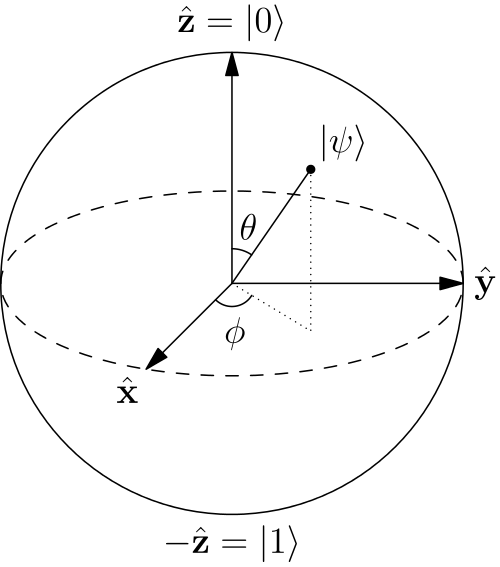
\includegraphics[width=0.35\textwidth]{500px-Bloch_Sphere_svg.png}
    \caption{Unit sphere $S^2$ with spherical coordinates $\theta$, $\phi$. }
    	\end{center}
    \end{figure}
   	\begin{equation}
		\ket{\psi} = \cos\frac{\theta}{2}e^{-i\phi}\ket{0}+\sin\frac{\theta}{2}e^{i\phi}\ket{1}
    \end{equation}
\end{frame}

%\subsection{Measurement}
\begin{frame}{Mathematics}
\textbf{Measurement} of \textbf{quantum states}
	\begin{itemize}
    	\item \textbf{Projection operator}: $\hat{P}_n = \ket{n}\bra{n}$, idempotent
        	\begin{equation}
            	\bra{n}\hat{P}_n\ket{\psi} = \alpha_n\
            \end{equation}
    	\item \textbf{Density operator} describes a quantum system in \textbf{mixed state} (statistical ensemble of several quatum states)
        	\begin{equation}\label{density}
            	\hat{\rho} = \sum_n p_n \ket{\psi_n}\bra{\psi_n}
            \end{equation}
         	Pure state only if $Tr(\hat{\rho}^2) = 1$ or $\hat{\rho}$ is idempotent.       
    \end{itemize}
\end{frame}

\begin{frame}{Mathematics}
\textbf{Measurement} of \textbf{quantum states}
	\begin{itemize}
    	\item \textbf{Expectation value}: Let $\hat{A}$ be an \textbf{observable} of a quantum system, assuming the ensemble is in mixed state such that each pure state $\ket{\psi_n}$ occurs with a probability $p_n$, the density operator is like in eqn.(\ref{density}). The expection value of the measurement calculates as
        \begin{equation}\begin{split}
\langle\hat{A}\rangle & =  \sum_n p_n\braket{\psi_n|\hat{A}|\psi_n}=\sum_n Tr\left(p_n\ket{\psi_n}\bra{\psi_n}\hat{A}\right)\\
	& = Tr\left(\sum_n p_n\ket{\psi_n}\bra{\psi_n}\hat{A}\right) = Tr\left(\hat{\rho}\hat{A}\right)
        \end{split}\end{equation}
    \end{itemize}
\end{frame}

\subsection{Several qubits}
\begin{frame}{Mathematics}
\textbf{Tensor product} in \textbf{Hilbert space}
	\begin{itemize}
    	\item Let $\mathcal{H}_j \subseteq \mathcal{H}$ be a Hilbert space and with basis vectors $\ket{n}_j \in \mathcal{H}_j$ representing a complete orthonormal system. Then, the Tensor product $\ket{ij}$ will be $\ket{ij}\in \mathcal{H}_i \bigotimes \mathcal{H}_j$
        \begin{equation}
     \ket{nm} := \ket{n}_i\ket{m}_j = \ket{n}_i\otimes\ket{m}_j  
        \end{equation}
        \item Example, using presentation of spins (2 Qubits)\\
        obtaining following set
\[ \lbrace\ket{0}\otimes\ket{0},\ket{0}\otimes\ket{1},\ket{1}\otimes\ket{0},\ket{1}\otimes\ket{1}\rbrace \]\\
\[\ket{01} = \ket{0}\ket{1}=\ket{0}_1\ket{1}_2=\ket{0}_1\otimes\ket{1}_2\]
    \end{itemize}
\end{frame}

\begin{frame}{Mathematics}
\textbf{Qubits}
	\begin{itemize}
    	\item \textbf{Superposition}: composition of 2 qubits\\
Consider $\ket{\vartheta}_1 = \alpha\ket{0}_1+\beta\ket{1}_1$, $\ket{\phi}_2 = \ket{1}_2$, $\alpha,\beta \in \mathbb{C}$ \\
\[\ket{\psi} = \ket{\vartheta\phi} = \left(\alpha\ket{0}_1+\beta\ket{1}_1\right)\ket{1}_2 =  \alpha\ket{01} + \beta\ket{11}  \]
		\item \textbf{Entanglement}: Quantum state is not reachable by tensor product. Examples:
		\begin{equation}\begin{split} \ket{\psi} & =  \frac{1}{\sqrt{|\alpha|^2+|\beta|^2}}\left(\alpha\ket{00} + \beta\ket{11}\right)   \\
\ket{\phi}_{\pm} & = \frac{1}{\sqrt{2}}\left(\ket{01}\pm\ket{10}\right)  
		\end{split}\end{equation}
    \end{itemize}
\end{frame}

\begin{frame}{Mathematics}
\textbf{Measurement of Spins} of m-qubits
	\begin{itemize}
    	\item Assuming observable operator $\hat{E}_j$ with $\lbrace j\in\mathbb{N} | 0 \leqslant j \leqslant m \rbrace$ \\
        Projection on standard basis $\lbrace\ket{0},\ket{1}\rbrace^n$
        \[\hat{E}_j\ket{n_0n_1\dots n_m} = n_j\ket{n_0n_1\dots n_m} \]
        \item Example: 2 qubits\\
        \begin{center}
        \begin{tabular}{|c|c|c|}
        	\hline
            quantum state $\ket{\psi}$ & measurement $\hat{E}_1$ & measurement $\hat{E}_2$ \\ 				\hline
            $\ket{01} $ & 0 & 1\\
            $\ket{10}-\ket{11}$ & 1 & $0\vee1$\\
            $\ket{00}+\ket{10}$ & $0 \vee 1$ & 0\\
            $\ket{00}+\ket{11}$ & $0 \vee 1$ & $0 \vee 1$\\
            \hline
        \end{tabular}\end{center}
	\end{itemize}
\end{frame}

\subsection{Quantum gates}
\begin{frame}{Mathematics}
\textbf{Unitary operations} with \textbf{gates}
	\begin{itemize}
    	\item To compute on quantum states, we will use unitary operations. Input qubits $\longrightarrow$ compute  $\longrightarrow$ output qubits (measurement).
        \item \textbf{Unitary operators} preserve the norm of the quantum system. It executes a rotation of $\ket{\psi}$ in spin-space \textbf{surface of Blochsphere}.
        \begin{equation}
\parallel\hat{U}\ket{\psi}\parallel=\parallel\ket{\psi}\parallel
        \end{equation}
        \item properties: $ \hat{U}^{\dagger} = \hat{U}^{-1}$ 
        	\begin{equation}
            	\hat{U}\hat{U}^{\dagger}=\hat{U}^{\dagger}\hat{U}=\hat{U}^{-1}\hat{U} = \hat{U}\hat{U}^{-1}=\hat{\mathbbm{1}} 
            \end{equation}
    \end{itemize}
\end{frame}

\begin{frame}{Mathematics}
\textbf{Not-gate}
	\begin{itemize}
    	\item A \textbf{not-gate} converts one basis state into another:\\     $\ket{0}\longrightarrow\ket{1}$ and $\ket{1}\longrightarrow\ket{0}$. Mathematically  written
        \begin{equation}
        \begin{split}
        \hat{N}\ket{0}=\ket{1} \\ \hat{N}\ket{1}=\ket{0}
        \end{split}
        \end{equation}
        With superposition $\ket{\psi}_{\pm}= \frac{1}{\sqrt{2}}\left( \ket{0}\pm \ket{1}\right) $ the output of the not-gate is
        \begin{equation}
        \hat{N}\ket{\psi}_{\pm}=\frac{1}{\sqrt{2}}\hat{N}\left( \ket{0}\pm \ket{1}\right)=\frac{1}{\sqrt{2}}\left(\ket{1}\pm\ket{0}\right)=\pm\ket{\psi}_{\pm}
        \end{equation}
    \end{itemize}
\end{frame}

\begin{frame}{Mathematics}
\textbf{Controlled not-gate}
	\begin{itemize}
    	\item A \textbf{controlled not-gate} takes effect on a 2-qubit state and only if the first qubit is in state $\ket{1}$ the second qubit becomes changed.
        \begin{equation}
        \hat{N}_c\ket{n}\ket{m} = \ket{n}\ket{(n+m)\mod 2}
        \end{equation}
        \item Examples:
        \begin{equation}
        \begin{split}
        \hat{N}_c\ket{00} & =\ket{00} \\
        \hat{N}_c\ket{11} & =\ket{10} \\
        \hat{N}_c\left(\frac{1}{\sqrt{2}}(\ket{00}\pm\ket{10})\right) & = \frac{1}{\sqrt{2}}(\ket{00}\pm\ket{11})
        \end{split}
        \end{equation}
    \end{itemize}
\end{frame}

\begin{frame}{Mathematics}
\textbf{Hadamard transform}
	\begin{itemize}
    	\item The Hadamard transform is needed to create superposition states out of basis states. It can be written as
        \begin{equation}
  \hat{H}\ket{n} = \frac{1}{\sqrt{2}}\sum_m (-1)^{nm}\ket{m}  
        \end{equation}
        \item the affect on basis states $\ket{0},\ket{1}$
        \begin{equation}\begin{split}
        \hat{H}\ket{0} & = \frac{1}{\sqrt{2}}(\ket{0}+\ket{1}) \\
        \hat{H}\ket{1} & = \frac{1}{\sqrt{2}}(\ket{0}-\ket{1})
        \end{split}\end{equation}
    \end{itemize}
\end{frame}

\subsection{Deutsch's problem}
\begin{frame}{Mathematics}
\textbf{Deutsch's problem}
	\begin{itemize}
    	\item Deutsch's algorithm for distinguishing between constant and balanced functions: For each arbitrary function $ f: \lbrace 0,1\rbrace \longrightarrow \lbrace 0,1\rbrace$, we define the unitary operation
        \begin{equation}
\hat{U}_f\ket{n}\ket{m} = \ket{n}\ket{(m+f(n))\mod 2}        
        \end{equation}
        \item using a quantum circuit which solves the problem:
\begin{align*}
 \Qcircuit @C=1em @R=.7em {
  \lstick{\ket{0}} & \qw & \gate{H} & \multigate{1}{U_f} & \gate{H}	& \meter & \cw \\
  \lstick{\ket{1}} & \qw     & \gate{H}             & \ghost{U_f}        & \qw
 }
\end{align*}
    \end{itemize}
\end{frame}

\begin{frame}{Mathematics}
\textbf{Deutsch's problem}
	\begin{itemize}
    	\item Compute with input $\ket{0}\ket{1} $
        \begin{equation}\begin{split}
\ket{01} & \rightarrow \frac{1}{2}(\ket{0}+\ket{1})(\ket{0}-\ket{1}) \\
	& \rightarrow \frac{1}{2}\left((-1)^{f(0)}\ket{0}+(-1)^{f(1)}\ket{1}\right)(\ket{0}-\ket{1}) \\
    & \rightarrow \frac{1}{2}\biggl[\left((-1)^{f(0)}+(-1)^{f(1)}\right)\ket{0} + \\ 
    & \quad + \left((-1)^{f(0)}-(-1)^{f(1)}\right)\ket{1}\biggr]\frac{1}{\sqrt{2}}(\ket{0}-\ket{1}) 
        \end{split}\end{equation}
        \item Measuring the first qubit, we find the outcome $\ket{0}$ with probability 1 if $f(0)=f(1)$ (\textbf{const.} func.) and the outcome $\ket{1}$ with expection value 1 if $f(0)\neq f(1)$ (\textbf{balanced} func.)
    \end{itemize}
\end{frame}

\subsection{No-cloning theorem}
\begin{frame}{Mathematics}
\textbf{No cloning theorem}
	\begin{itemize}
    \item Important for quantum informatics, as no classical error correction codes are possible-
    \item Is the basis for quantum cryptography.
    \item Proof: Assuming perfect copies by an unitary operation of arbitrary qubits. 2 arbitrary quantum states $\ket{\phi}, \ket{\psi} \rightarrow$ transferred to independent state $\ket{\lambda}$ \\
    Copying:
    \begin{align}
\hat{U}(\ket{\phi}\otimes\ket{\lambda}) & = \ket{\phi}\otimes\ket{\phi} \\
\hat{U}(\ket{\psi}\otimes\ket{\lambda}) & = \ket{\psi}\otimes\ket{\psi}
    \end{align}
	\end{itemize}
\end{frame}

\begin{frame}{Mathematics}
\textbf{No cloning theorem}
	\begin{itemize}
		\item Scalar product:
            \begin{align}\begin{split}
\braket{(\phi\otimes\lambda)|(\psi\otimes\lambda)} & = \braket{(\phi\otimes\lambda)|\hat{U}^{\dagger}\hat{U}|(\psi\otimes\lambda)} \\
& = \braket{(\phi\otimes\phi)|(\psi\otimes\psi)}
			\end{split}\end{align}
            \begin{align}\begin{split}
\braket{(\phi\otimes\lambda)|(\psi\otimes\lambda)} & = \braket{\phi|\psi}\braket{\lambda|\lambda} = \braket{\phi|\psi} \\
\braket{(\phi\otimes\phi)|(\psi\otimes\psi)} & = \braket{\phi|\psi} \braket{\phi|\psi} = \braket{\phi|\psi}^2
            \end{split}\end{align}
        \item So $\braket{\phi|\psi}^2 = \braket{\phi|\psi}$, $\Rightarrow$ solutions: $\braket{\phi|\psi} = 0$ or $\braket{\phi|\psi} = 1$ \\ $\Rightarrow$ $\ket{\phi}$ is an orthogonal state of $\ket{\psi}$ or $\ket{\phi} = \ket{\psi}$.
        \item It is not possible to copy \textbf{arbitrary states}. 
	\end{itemize}
\end{frame}

% Kapitelframes - nur ein zentriertel Titel
%-----------------------------------------------------------------------------
\section{Algorithms}
\chapterframe{Algorithms}

\begin{frame}{Algorithms}
	\begin{itemize}
		\item Quantum algorithms use a number of techinques, e.g.
			\begin{itemize}
				\item Quantum Fourier Transform (QFT)
				\item Amplitude Amplification
				\item Quantum Walks
			\end{itemize}
		\item These often take $\Omega(2^n)$ time on classical computers,
		\item but often only $O(n^k)$ on quantum computers*.
			\begin{itemize}
				\item * given certain assumptions.
			\end{itemize}
	\end{itemize}
\end{frame}

\begin{frame}{Fourier Transform}
	\begin{itemize}
		\item The Fourier series decomposes a function $f : \mathbb{R} : \rightarrow \mathbb{C}$  into periodic components.
    
    \begin{center}
    	\includegraphics<1>{ft_1.png}
    	\includegraphics<2->{ft_2.png}
    \end{center}
    
    \item<3-> Any function $f$ can be approximated by a number of sinusoidal functions. 
    
    \item<4-> The {\em discrete} Fourier Transform (DFT) does the same, but operates on a list $[x_1,\dots,x_n] $ of equally spaced samples.
    
	\end{itemize}
        
\end{frame}

\begin{frame}{Quantum Fourier Transform}
	\begin{itemize}
		\item DFT is computed as $dft : (x_1,\dots,x_n) \mapsto (a_1,\dots,a_{\frac{n}{2}},b_1,\dots,b_{\frac{n}{2}})$ with
        $$
        	a_m = \sum\limits_{i=0}^{n-1} \frac{2\pi}{n} f(x_i) \cos(mx_i)
        $$
        $$
        	b_m = \sum\limits_{i=0}^{n-1} \frac{2\pi}{n} f(x_i) \sin(mx_i)
        $$
        
        \item QFT, equivalently, maps quantum states $\ket{x_1 x_2 \dots x_n}$.
        
	\end{itemize}
\end{frame}

\begin{frame}{Quantum Fourier Transform}
	\begin{itemize}
        \item For simplicity, let us assume $n = 2^m$ for some $m$.
        \item $\ket{X} = \ket{x_1\dots x_n} = \ket{x_1} \otimes \dots \otimes \ket{x_n}$
              where
              $X = x_1 2^{n-1} + \dots + x_n 2^0$
        \item QFT can be implemented as follows:
        	  $$
              	\ket{X} \mapsto \frac{1}{\sqrt{N}} \left( \mt{vec}(n) \otimes \dots \otimes \mt{vec}(1) \right)
              $$
              where
              $$
              	\mt{vec}(i) = \ket{0} + e^{2 \phi i \mt{exp}(i)} \ket{1}
              $$
              $$
              	\mt{exp}(i) = \sum\limits_{k = i}^{n} \frac{x_k}{2^k} = \frac{x_i}{2} + \dots + \frac{x_n}{2}
              $$
        \item $\left( \mt{vec}(n) \otimes \dots \otimes \mt{vec}(1) \right)$ is the tensor product of n single-qubit operations.
        \item Each operation canbe implemented using a Hadamard gate.
	\end{itemize}
\end{frame}

\subsection{Shor's algorithm}

\begin{frame}{Shor's Algorithm}{Quantum Fourier Transform}
	\begin{definition}[Integer factorization (IF)]
		$\texttt{factor} : \mathbb{N} \rightarrow \mt{Set}[\mathbb{N} \times \mathbb{N}]$\\
        	Input: $n \in \mathbb{N}$\\
        	Output: $P \subseteq \mathbb{N} \times \mathbb{N}$ s.t. $[\forall (p,e) \in P]\ \mt{prime}(p)$ and $\prod\limits_{(p,e) \in P} p^e = n$
	\end{definition}
    
    \begin{example}
       $2448 = 2^4 * 3^2 * 17^1\ \ \Rightarrow\ \ 
       \texttt{factor}(2448) = \{(2,4), (3,2), (17,1)\}$
    \end{example}

	\begin{itemize}
		\item Best known classical algorithm: generalized prime number sieve (GPNS).
			\begin{itemize}
				\item $O(e^{1.9 \log(n)^{\frac{1}{3}} (\log\log(n))^{\frac{2}{3}}}) = O(e^{f(n)})$ for sub-exponential $f$.
			\end{itemize}

		\item \textbf{Shor's algorithm} runs in \textbf{polylogarithmic} time.
			\begin{itemize}
				\item $O(\log(n)^3)$
			\end{itemize}
	\end{itemize}
\end{frame}

\begin{frame}[fragile]{Shor's Algorithm}{Quantum Fourier Transform}       
	\begin{itemize}
    	\item Shor's algorithm has a \textbf{classical} and a \textbf{quantum} part.
    \end{itemize}
    
    \begin{code}[Classical part]
    	\begin{flushleft}
        	\vspace{-0.5cm}
			\begin{lstlisting}[mathescape, language=Haskell]
				//Definitions
				let a = random number < n
				    func(x) = $a^x \mod n$
				    r = $\textbf{period(func)}$ //use QFT
				
				//We correctly guessed a factor
				case gcd(a,n) $\neq 1$     $\Rightarrow$ return a
				
				//We use the quantum part (period)
				case r is odd      $\Rightarrow$ repeat
				case $a^{\frac{r}{2}} \mod n = n - 1$ $\hspace{-0.1cm}\Rightarrow$ repeat
				case otherwise     $\Rightarrow$ return gcd($a^{\frac{r}{2}} \pm 1$, n)
			\end{lstlisting}
		\end{flushleft}
    \end{code}
\end{frame}

\begin{frame}[fragile]{Shor's Algorithm}{Quantum Fourier Transform}       
	\begin{itemize}
    	\item \texttt{period}(x) is the quantum part and uses QFT to determine the period of $a^x \mod n$.
        \item Using number-theoretical results (the Chinese Remainder Theorem and Bézout's identity), we can derive factors from the period.\\
        
        \item The function problem \textbf{IF} can be reduced to a decision problem thus:
        
      \begin{definition}[Integer factorization decision (IF-dec)]
          $\texttt{hasFactor} : \mathbb{N} \rightarrow \mathbb{N} \rightarrow \mt{Bool}$\\
              Input: $n \in \mathbb{N}$ and bound $k \in \mathbb{N}$\\
              Output: true iff $n$ as a non-trivial factor $<k$.
      \end{definition}
      
      \item Through binary search on $k$, we can find the factors of $n$ with polynomially many calls to \texttt{hasFactor}.
    \end{itemize}
\end{frame}

\subsection{Grover's algorithm}

\begin{frame}{Grover's Algorithm}{Amplitude Amplification}
	\begin{definition}[Unsorted search]
		$\texttt{elem} : T \rightarrow \mt{List}[T] \rightarrow \mt{Bool}$\\
        	Input: $e \in T, list \in \mt{List}[T]$\\
        	Output: $\mt{true}$ iff $e$ occurs in $list$. 
	\end{definition}
    
    \begin{example}
       $elem\ 5\ [2,1,7,3,9] = \mt{false}$\\
       $elem\ 5\ [2,1,7,3,\textbf{5},9] = \mt{true}$
    \end{example}

	\begin{itemize}
		\item Classical search takes $\Theta(n)$ time ($n = \mt{length}(list)$): one has to iterate through the whole list.

		\item \textbf{Grover's algorithm} takes only $O(\sqrt{n})$ steps.
	\end{itemize}
\end{frame}

\begin{frame}[fragile]{Grover's Algorithm}{Amplitude Amplification}       
    \begin{code}
    	\begin{flushleft}
        	\vspace{-0.5cm}
			\begin{lstlisting}[mathescape, language=Haskell]
				initialize the system S to the distribution
				$\left( \frac{1}{\sqrt{n}}, \cdots , \frac{1}{\sqrt{n}} \right)$
                   
				repeat $O(\sqrt{n})$ times:
				   case C(S) = 1 $\Rightarrow$ rotate the phase by $\pi$ radians
				   case C(S) = 0 $\Rightarrow$ leave S unaltered
                   
				   apply the matrix D where
				      $m = \frac{2}{n}$
				      $D =
                      	\left[
                        	\begin{array}{l c c r}
                            	(-1 + m) & m        & \dots & m\\
                                m        & (-1 + m) & \dots & m\\
                                \vdots   &          & \ddots & \vdots\\
                                m        & \dots    & m     & (-1 + m)
                            \end{array}
                        \right]$
			\end{lstlisting}
		\end{flushleft}
    \end{code}
\end{frame}

\begin{frame}{Grover's Algorithm}{Amplitude Amplification}       
    \begin{itemize}
    	\item $D$ can be implemented as $D = WRW$ where $R$ is the rotation matrix and $W$ is the Welsh-Hadamard matrix, defined as
        $$
        	W_{ij} = 2^{\frac{-n}{n}} * (-1)^{\mt{bit}(i)\ \cdot\ \mt{bit}(j)}
            \quad
            \quad
        	R = \left[
            \begin{array}{l l l l r}
            	1 & 0  &  0 & \dots & 0\\
                0 & -1 &  0 & \dots & 0\\
                0 & 0  & -1 & \dots & 0\\
                \vdots & & & \ddots & \vdots\\
                0 & \multicolumn{2}{c}{\dots}  & 0 & -1
            \end{array}
            \right]
        $$
    \end{itemize}
\end{frame}

\begin{frame}{Grover's Algorithm}{Amplitude Amplification}       
    \begin{itemize}
    	\item In each iteration, the amplitude of the desired state is increased by $O(\frac{1}{\sqrt{n}})$.
        \item After $O(\sqrt{n})$ iterations, the amplitude of the desired state is 1.
        \item In the end, the system is sampled. If $\exists S_{\mt{target}}$ s.t. $C(S_{\mt{target}}) = 1$ then $P(S = S_{\mt{target}}) \geq \frac{1}{2}$.
    \end{itemize}
\end{frame}

\begin{frame}{Quantum Walks}
	\begin{itemize}
      \item A (discrete-time) random walk in n dimensions is an infinite series $[(0,\dots,0), (x_1^1,\dots,x_n^1), (x_1^2,\dots,x_n^2),\dots]$ where, for all $k \in \mathbb{N}$, $x_i^k$ is a sample of the random variable $X_i$.
      \item The random variables $X_1,\dots,X_n$ are pairwise independent and $P(X_i = 1) = P(X_i = -1) = 0.5$ for $1 \leq i \leq n$.
   	\end{itemize}
    
    \begin{center}
    	\includegraphics<2>[width=200pt]{1dimRandomWalk.png}
    \end{center}
\end{frame}

\begin{frame}{Quantum Walks}
	\begin{itemize}
      \item With random walks, the system is in state $(s_1,\dots,s_n)$  at time $t$ with a certain probability.
      \item With Quantums walks, the system is in a superposition of states.
   	\end{itemize}
\end{frame}


\subsection{Element distinctness problem}


\begin{frame}{Element Distinctness Problem}{Quantum walks}
	\begin{definition}[All elements distinct]
		$\texttt{distinct} : \mt{List}[T] \rightarrow \mt{Bool}$\\
        	Input: $list \in \mt{List}[T]$\\
        	Output: $\mt{true}$ iff there are no $i,j$ s.t. $i \neq j$ and $list[i] = list[j]$. 
	\end{definition}
    
    \begin{example}
       $distinct\ [2,1,7,3,9] = \mt{true}$\\
       $distinct\ [2,\textbf{1},7,3,\textbf{1},9] = \mt{false}$
    \end{example}

	\begin{itemize}
		\item Classical search takes $\Theta(n \log(n))$ time: sort the list and iterate, looking for identical consecutive elements.

		\item \textbf{Andris Ambainis} provides an $O(n^{\frac{2}{3}})$ algorithm.
	\end{itemize}
\end{frame}

\begin{frame}[fragile]{Element distinctness problem}{Quantum walks}       
    \begin{code}
    	\begin{flushleft}
        	\vspace{-0.5cm}
			\begin{lstlisting}[mathescape, language=Haskell]
				//Definitions
				let ind = [1,$\dots$,length(list)]
				    r = $n^\frac{2}{3}$
				    $G = (V,E,mark)$ with $|V| = \binom{n}{r} + \binom{n}{r+1}$
				       where
				          $v_S \in V \Leftrightarrow S \subseteq ind$ with $r \leq |S| \leq r+1$;
				          $(v_S,v_T) \in E \Leftrightarrow T = S \cup \{i\}$ for some $i \in list$
				          $mark(v_S) = 1 \Leftrightarrow \{i,j\} \in ind \wedge list[i] = list[j]$
                          
				find_marked_vertex(G)
			\end{lstlisting}
		\end{flushleft}
    \end{code}
\end{frame}

\begin{frame}[fragile]{Element distinctness problem}{Quantum walks}       
    \begin{code}[Finding a marked vertex]
    	\begin{flushleft}
        	\vspace{-0.5cm}
			\begin{lstlisting}[mathescape]
				1. start with a uniform superposition over $V$
				2. Repeat $(N/r)$ times:
				      2.1 Apply $\ket{S}\ket{y}\ket{list} \rightarrow -\ket{S}\ket{y}\ket{list}$
				          for a marked S
				          $x \in [1,\dots,m]^r$
				          $y \in ind - S$
				      2.2 Perform $\sqrt{r}$ steps of a quantum walk
				          through G.
			\end{lstlisting}
		\end{flushleft}
    \end{code}
    
    $m$ is reused accross queries: if we move from $v_S$ to $v_T$, we set $m$ to $|T - S|$.
\end{frame}

\begin{frame}{BQP and NP}
	\begin{itemize}
    	\item The algorithms just discussed all lie in \textbf{BQP}:
        
        \begin{definition}[Bounded error quantum polynomial time]
        	A language $X \in \textbf{BQP}$ iff $\exists f : \mt{List}[\mt{Qubit}] \rightarrow \mt{Bit}$ for $X$ s.t.
            \begin{enumerate}
            	\item $f$ takes $n$ qubits of input,
            	\item $f$ runs in $O(n^k$ time (for a constant $k$),
                \item $x \in X \Rightarrow P(f(x) = 1) \geq \frac{2}{3}$,
                \item $x \notin X \Rightarrow P(f(x) = 0) \geq \frac{2}{3}$.
            \end{enumerate}
        \end{definition}
        
        \item \textbf{BQP} is the quantum-analogue of \textbf{BPP}:
        
                \begin{definition}[Bounded error polynomial time]
        	A language $X \in \textbf{BQP}$ iff $\exists f : \mt{List}[\mt{Bit}] \rightarrow \mt{Bit}$ for $X$ s.t.
            \begin{enumerate}
            	\item $f$ takes $n$ {\em bits} of input,
                \item $f$ may make use of a true random number generator,
            	\item $f$ runs in $O(n^k$ time (for a constant $k$),
                \item $x \in X \Rightarrow P(f(x) = 1) \geq \frac{2}{3}$,
                \item $x \notin X \Rightarrow P(f(x) = 0) \geq \frac{2}{3}$.
            \end{enumerate}
        \end{definition}
    \end{itemize}
\end{frame}

\begin{frame}{BQP and NP}
	\begin{itemize}
    	\item $\textbf{P} \subseteq \textbf{BPP} \subseteq \textbf{BQP} \subseteq \textbf{PSPACE}$
        \item However, both $\textbf{BQP} \stackrel{?}{\subseteq} \textbf{NP}$ and $\textbf{NP} \stackrel{?}{\subseteq} \textbf{BQP}$ are unknown.
        \item Shor's algorithm solves the \textbf{NP}-problem \textbf{IF}, but $\textbf{IF} \stackrel{?}{\in} \textbf{NP-complete}$ is not known.
        \item Hence, it is not known whether quantum computers can actually solve the class \textbf{NP} in polynomial time.
    \end{itemize}
\end{frame}

\begin{frame}
	\begin{itemize}
    	\item Sources:
        	\begin{itemize}
            	\item Shor's algorithm: \url{http://arxiv.org/abs/quant-ph/0303175}
                \item Grover's algorithm: \url{http://arxiv.org/abs/quantph/9605043}
                \item Ambainis's algorithm: \url{http://arxiv.org/abs/quantph/0311001}
            \end{itemize}
    \end{itemize}
\end{frame}

% Kapitelframes - nur ein zentriertel Titel
%----------------------------------------------------------------------------
%
%

\section{How to buld a quantum computer?}
\chapterframe{How to build a quantum computer?}


\begin{frame}{Requirements for a quantum computer}
 \begin{itemize}
   \item A scalable physical system with well characterized quibits
    \item The ability to initialize the state of the qubits to a simple fiducial state such as $\bra{000\dots}$
    \item Long relevant decoherence times, much longer than the gate operation time
    \item A "universal" set of quantum gates
    \item A qubit-specific measurement capability
 
 \end{itemize}
\end{frame}

\begin{frame}{Problems}

 \begin{itemize}
 
  \item \textbf{Relaxation} - falling back to state with lower energy.
  
  \item \textbf{Dekoherence} - superposition gets lost through external influence.
 
 \end{itemize}


\end{frame}

\begin{frame}{Possible Technological Candiates}
 \begin{itemize}
  \item Bose-Einstein condensate (BEC)
  \item Ion Traps
  \item Super-conducting qubits
  \item Cold-atom optical lattices
  \item NV-centers in diamonds
  \item Semiconductor quantum dots
 \end{itemize}

\end{frame}

\begin{frame}{Bose-Einstein condensate (BEC)}

\begin{itemize}
  \item Temperature very close to 0 K
  \item Quantum effects manifest on macroscopic level
  \item Same quantum state over multiple atom
  \item Two-component BCE for qubits.
\end{itemize}


\end{frame}

\begin{frame}{Ion Traps}

\begin{itemize}
	\item Long storage of state
    \item Ions in vacuum 
    \item Initialisation with optical pumping
    \item Measurement via laser
    \item Operations 97\% successful
\end{itemize}    
    
\end{frame}


\begin{frame}{Super-conducting qubits}

\begin{itemize}
 \item Super-conducting circuit
 \item With Josephson junction
 \item Initialisation with microwaves
 
\end{itemize}

\end{frame}

\begin{frame}{Cold-atom in opcial lattices}

\begin{itemize}
 \item Grid of laser beams
 \item Periodic potential traps neutral atoms

\end{itemize}

	\begin{center}
		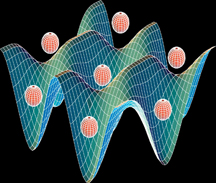
\includegraphics[scale=0.8]{optlat.jpg}
	\end{center}


\end{frame}


\begin{frame}{NV-centers in diamonds}

\begin{itemize}
 \item Nitrogen (N) replaces carbon (C) in diamond
 \item Initialisation with laser beams
 \item Diamond structure isolates qubits from external influence
 \item No cooling required
\end{itemize}

\end{frame}


\begin{frame}{Semiconductor quantum dot}

\begin{itemize}
  \item $10^3$ to $10^9$ atoms
  \item Electrons cannot move
  \item Discrete electronic state
  \item Qubit as spin of electron
  \item Initialisation with magnetic fields  
\end{itemize}


\end{frame}

\section{Recent developments}
\chapterframe{Recent developments}

\begin{frame}{Recent developments}
%(neue papers)

	\begin{itemize}
 		\item At the TU:
        	\begin{itemize}
            	\item \url{http://www.tuwien.ac.at/aktuelles/news_detail/article/8744/}
            \end{itemize}
     \end{itemize}


\end{frame}




\end{document}
